% Created 2024-06-22 Sat 19:55
% Intended LaTeX compiler: pdflatex
\documentclass[11pt]{article}
\usepackage[utf8]{inputenc}
\usepackage[T1]{fontenc}
\usepackage{graphicx}
\usepackage{longtable}
\usepackage{wrapfig}
\usepackage{rotating}
\usepackage[normalem]{ulem}
\usepackage{amsmath}
\usepackage{amssymb}
\usepackage{capt-of}
\usepackage{hyperref}
\usepackage[a4paper,left=1cm,right=1cm,top=1cm,bottom=1cm]{geometry}
\usepackage[american]{babel}
\usepackage{enumitem}
\usepackage{float}
\usepackage[sc]{mathpazo}
\linespread{1.05}
\renewcommand{\labelitemi}{$\rhd$}
\setlength\parindent{0pt}
\setlist[itemize]{leftmargin=*}
\setlist{nosep}
\author{Marcio Woitek}
\date{}
\title{TSP Basics}
\hypersetup{
 pdfauthor={Marcio Woitek},
 pdftitle={TSP Basics},
 pdfkeywords={},
 pdfsubject={},
 pdfcreator={Emacs 29.3 (Org mode 9.6.24)}, 
 pdflang={English}}
\begin{document}

\maketitle
\thispagestyle{empty}
\pagestyle{empty}

Problems 1 and 2 are related to the graph below. Black edges have weight 1, and
red edges have weight 2.
\begin{figure}[H]
  \centering
  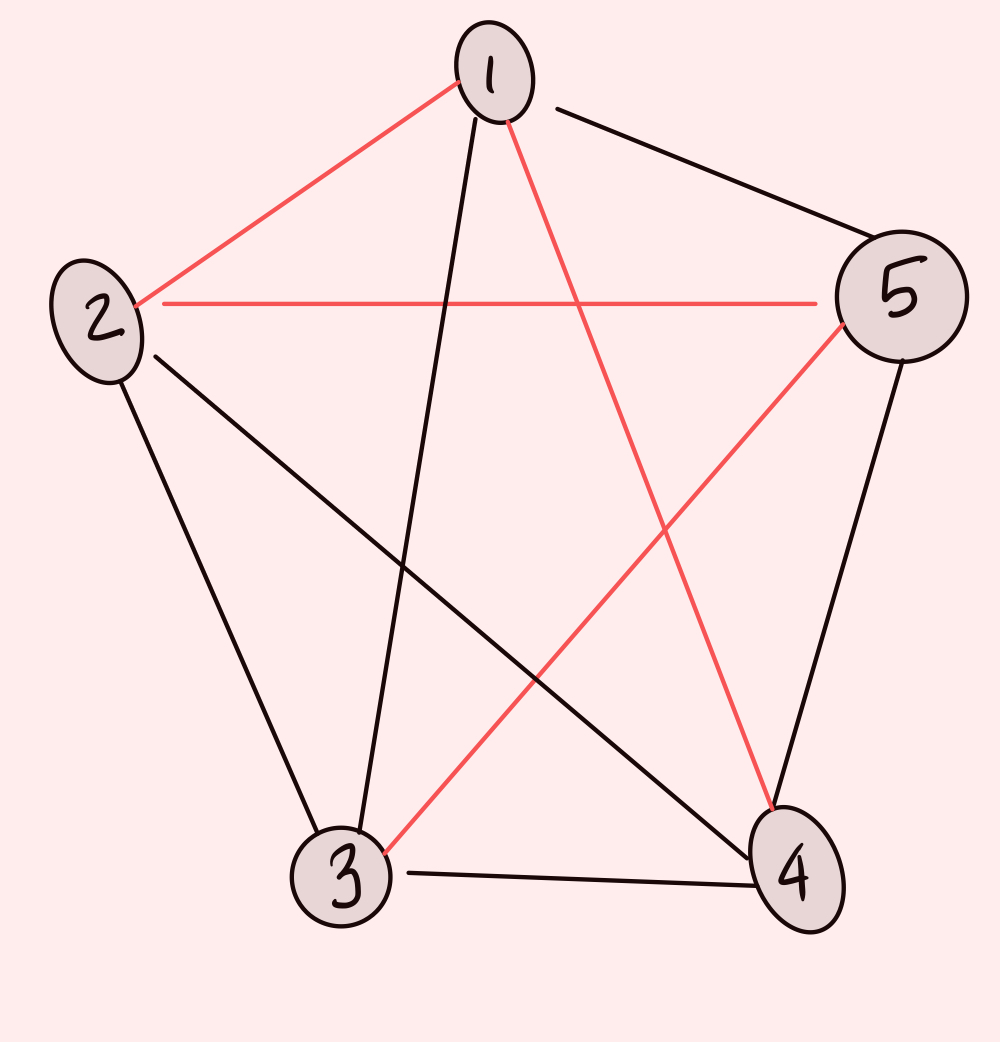
\includegraphics[scale=0.15]{held_karp_graph.jpeg}
  \caption{TSP instance}
\end{figure}

\section*{Problem 1}
\label{sec:org5e485f4}
\begin{itemize}
\item There is a TSP tour whose cost is 5, i.e., it involves only the black edges in
the graph.
\item The sequence of vertices 1, 2, 3, 4, 5, 1 (1 is the start/end point) is a
valid TSP tour of cost 6.
\end{itemize}

\section*{Problem 2}
\label{sec:org77a526f}
\textbf{Answer: True}

\section*{Problem 3}
\label{sec:orga3f939b}
This problem is related to the following graph:
\begin{figure}[H]
  \centering
  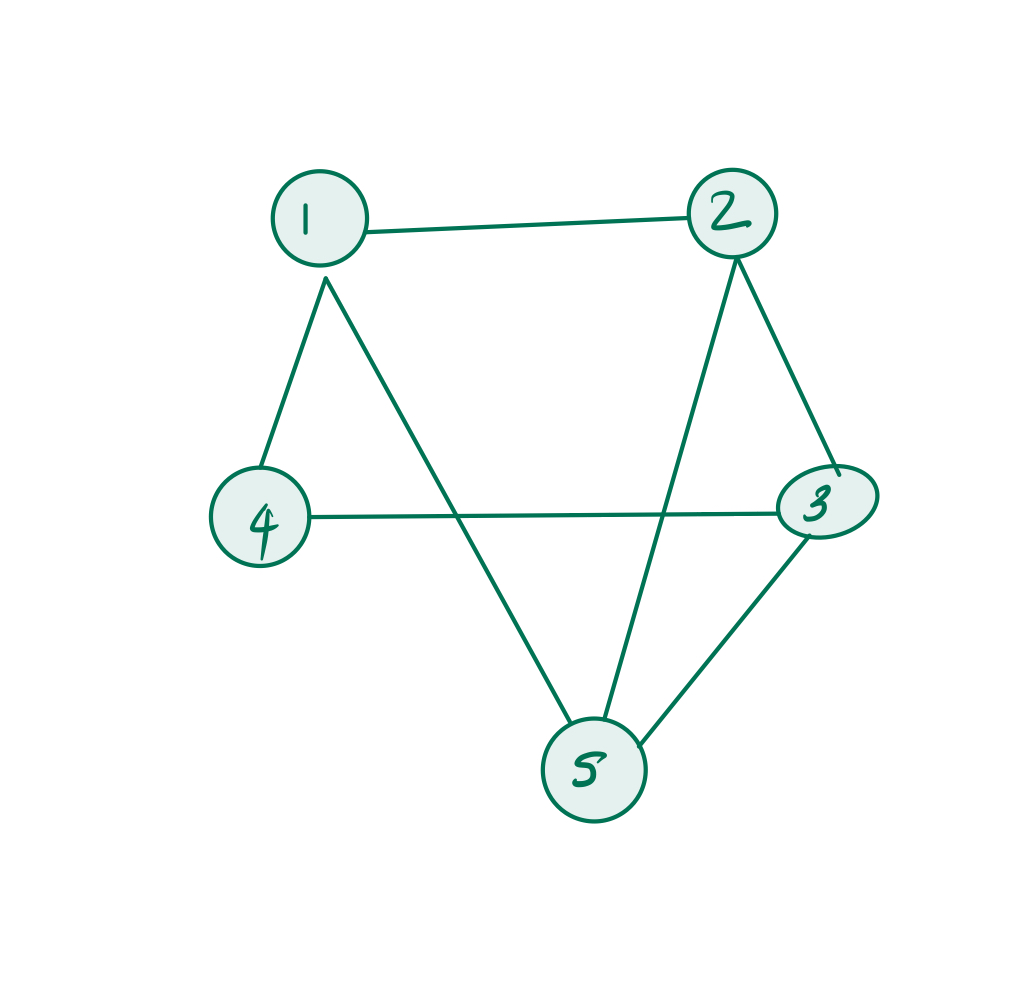
\includegraphics[scale=0.2]{ham_cycle.jpeg}
  \caption{Graph for question on Hamiltonian cycles}
\end{figure}

\begin{itemize}
\item The reduction will need to assign a weight of 1 to each edge in the original
graph and add the missing edges \((4,5)\), \((1,3)\) and \((2,4)\) with some weight
\(W>1\).
\item Once we reduce to the TSP, we conclude the presence of a Hamiltonian cycle if
the optimal TSP tour has weight 6.
\item Let \(W>1\) be the weight given to the missing edges that we will need to add
back for the reduction to the TSP. The optimal TSP tour cost will be at least
\(5+W\) if there is no Hamiltonian cycle.
\end{itemize}
\end{document}
